\newpage
\section{Systematische Literaturrecherche} \label{sec:Systematische Literaturrecherche}

Die systematische Literaturrecherche zum Stand der Forschung orientiert sich am \enquote{iterative Review-Ansatz} nach \textcite[S. 208--209]{brocke_StandingShouldersGiantsChallengesRecommendationsLiteratureSearchInformationSystemsResearch_2015}, der mit einer initialen Recherche startet und sich iterativ vertieft. Für die Struktur und Dokumentation sind ausgewählte Methoden der \ac{PRISMA} 2020 Richtlinien zugrunde gelegt (\autoref{tab:Ausgewählte Methoden der PRISMA 2020 Richtlinien}). \ac{PRISMA} gewährleistet hierbei einen transparenten, reproduzierbaren Prozess und verbessert die Berichtqualität \parencite[S. 1, 6]{page_PRISMA2020Statementupdatedguidelinereportingsystematicreviews_2021}.

\begin{longtable}{L{0.3\textwidth}L{0.7\textwidth}}
    \caption{Ausgewählte Methoden der PRISMA 2020 Richtlinien}
    \label{tab:Ausgewählte Methoden der PRISMA 2020 Richtlinien} \\
    \toprule
    \textbf{Methode} & \textbf{Beschreibung} \\
    \midrule
    \endfirsthead
    \multicolumn{2}{l}{\textit{Tabelle \thetable\ (Fortsetzung)}} \\
    \toprule
    \textbf{Methode} & \textbf{Beschreibung} \\
    \midrule
    \endhead
    \midrule
    \multicolumn{2}{r}{\textit{Fortsetzung auf nächster Seite}} \\
    \endfoot
    \bottomrule
    \multicolumn{2}{p{\linewidth}}{\textit{Anmerkung.} In Anlehnung an \textcite[S. 4]{page_PRISMA2020Statementupdatedguidelinereportingsystematicreviews_2021}.} \\
    \endlastfoot
    Ein- und Ausschlusskriterien & Ein- und Ausschlusskriterien für die Überprüfung. \\
    \midrule
    Suchstrategie & Vollständigen Suchstrategie für alle Datenbanken, Websites einschließlich aller verwendeten Filter. \\
    \midrule
    Selektionsprozess & Methoden an, die verwendet wurden, um zu entscheiden, ob eine Studie die Einschlusskriterien der Überprüfung erfüllt. \\
\end{longtable}

\pagebreak

Die in \autoref{tab:einausschlusskriterien} dargestellten Ein- und Ausschlusskriterien gewährleisten eine transparente, nachvollziehbare und zielgerichtete Auswahl relevanter wissenschaftlicher Quellen.

\begin{longtable}{L{3cm}L{4cm}L{4cm}L{3cm}}
    \caption{Ein- und Ausschlusskriterien für die systematische Literaturrecherche}
    \label{tab:einausschlusskriterien} \\
    \toprule
    \textbf{Kategorie} & \textbf{Einschluss} & \textbf{Ausschluss} & \textbf{Begründung} \\
    \midrule
    \endfirsthead
    \multicolumn{4}{l}{\textit{Tabelle \thetable\ (Fortsetzung)}} \\
    \toprule
    \textbf{Kategorie} & \textbf{Einschluss} & \textbf{Ausschluss} & \textbf{Begründung} \\
    \midrule
    \endhead
    \midrule
    \multicolumn{4}{r}{\textit{Fortsetzung auf nächster Seite}} \\
    \endfoot
    \bottomrule
    \multicolumn{4}{p{\linewidth}}{\textit{Anmerkung.} Eigene Darstellung.} \\
    \endlastfoot
    Thematischer Fokus &
    \ac{SSI} und dezentrale Identitätslösungen;
    Blockchain-basierte Identitätsmanagementsysteme;
    \ac{PQC} und quantensichere Algorithmen;
    Sicherheit und Compliance in \ac{KRITIS};
    \ac{DSR}-Methodik in IT/Informationssystemen;
    Kryptoagilität und kryptografische Migration & 
    Identitätsmanagement ohne Bezug zu \ac{SSI} oder Blockchain;
    Klassische \ac{PKI} ohne \ac{PQC}-Bezug;
    Kryptografie ohne Post-Quantum-Relevanz;
    Arbeiten ohne Bezug zu \ac{KRITIS} oder ohne sicherheitskritischen Kontext;
    Nicht-\ac{DSR}-basierte Entwicklungsansätze & 
    Fokussierung auf die Forschungsfragen und relevante technologische, methodische und regulatorische Aspekte. \\
    \midrule
    Zeitrahmen & 2015 bis heute & Vor 2015 & Berücksichtigung aktueller technologischer Entwicklungen (Blockchain, \ac{PQC}, \ac{SSI}) und regulatorischer Anforderungen. \\
    \midrule
    Publikationstypen & 
    Peer-reviewed Journalartikel;
    Konferenzbeiträge anerkannter Fachgesellschaften (z. B. IEEE, ACM, IFIP); Preprints;
    Offizielle Standards und Empfehlungen (z. B. \ac{NIST}, W3C, \ac{BSI});
    Whitepaper etablierter Organisationen;
    Dissertationen und anerkannte Fachbücher & 
    Blogposts, Forenbeiträge, Marketingmaterial;
    Populärwissenschaftliche Artikel ohne wissenschaftliche Fundierung;
    Unveröffentlichte Manuskripte ohne Peer-Review;
    Seminar- und Abschlussarbeiten ohne wissenschaftliche Begutachtung & 
    Sicherstellung wissenschaftlicher Qualität, Nachvollziehbarkeit und Relevanz der Quellen für die Masterarbeit; Da das Forschungsthema aktuell noch sehr neu ist und die einschlägige Fachliteratur teilweise noch nicht den Peer-Review-Prozess durchlaufen hat, werden auch Preprints in die Analyse einbezogen. Preprints ermöglichen eine zeitnahe Verfügbarkeit aktueller Forschungsergebnisse, was insbesondere bei diesem innovativen von großer Bedeutung ist. \\
    \midrule
    Sprache & Deutsch; Englisch & Andere Sprachen als Deutsch und Englisch & Gewährleistung der Verständlichkeit und Zugänglichkeit für den deutsch- und englischsprachigen Forschungskontext. \\
    \midrule
    Zugänglichkeit & Verfügbare Volltexte & Nicht verfügbare Volltexte & Ermöglichung einer gründlichen Analyse und Bewertung der Inhalte. \\
\end{longtable}

\autoref{tab:suchstrategie} stellt ausgewählte methodische Schritte zur Entwicklung einer Suchstrategie nach \textcite[S. 532]{bramer_SystematicApproachSearchingefficientcompletemethoddevelopliteraturesearches_2018} dar, an denen sich diese Seminararbeit orientiert.

\begin{longtable}{L{0.1\textwidth}L{0.9\textwidth}}
    \caption{Überblick über die Entwicklung der Suchstrategie}
    \label{tab:suchstrategie} \\
    \toprule
    \textbf{Schritt} & \textbf{Beschreibung} \\
    \midrule
    \endfirsthead
    \multicolumn{2}{l}{\textit{Tabelle \thetable\ (Fortsetzung)}} \\
    \toprule
    \textbf{Methode} & \textbf{Beschreibung} \\
    \midrule
    \endhead
    \midrule
    \multicolumn{2}{r}{\textit{Fortsetzung auf nächster Seite}} \\
    \endfoot
    \bottomrule
    \multicolumn{2}{p{\linewidth}}{\textit{Anmerkung.} In Anlehnung an \textcite[S. 532]{bramer_SystematicApproachSearchingefficientcompletemethoddevelopliteraturesearches_2018}.} \\
    \endlastfoot
    1  & Identifikation relevanter Schlüsselkonzepte \\
    \midrule
    2  & Identifikation relevanter Keywords \\
    \midrule 
    3  & Erstellung einer strukturierten Suchanfrage mit Booleschen Operatoren \\
    \midrule
    4  & Auswahl geeigneter Datenbanken \\
    \midrule
    5  & Übersetzung der Suchanfrage für verschiedene Datenbanken \\
\end{longtable}

\paragraph*{Identifikation relevanter Schlüsselkonzepte}

Im ersten Schritt wird eine präzise Identifikation und Abgrenzung zentraler Schlüsselkonzepte vorgenommen (\autoref{tab:Abgrenzung zentraler Schlüsselkonzepte}).

\begin{longtable}{L{4cm}L{10cm}}
    \caption{Abgrenzung zentraler Schlüsselkonzepte}
    \label{tab:Abgrenzung zentraler Schlüsselkonzepte} \\
    \toprule
    \textbf{Schlüsselkonzept} & \textbf{Erläuterung} \\
    \midrule
    \endfirsthead
    \multicolumn{2}{l}{\textit{Tabelle \thetable\ (Fortsetzung)}} \\
    \toprule
    \textbf{Schlüsselkonzept} & \textbf{Erläuterung} \\
    \midrule
    \endhead
    \midrule
    \multicolumn{2}{r}{\textit{Fortsetzung auf nächster Seite}} \\
    \endfoot
    \bottomrule
    \multicolumn{2}{p{\linewidth}}{\textit{Anmerkung.} Basierend auf \textcite[S. 2]{solavagione_TransitionSelfSovereignIdentityPostQuantumCryptography_2025}, \textcite{nationalinstituteofstandardsandtechnologyus_ModulelatticebasedKeyencapsulationMechanismstandard_2024,nationalinstituteofstandardsandtechnologyus_ModulelatticebasedDigitalSignaturestandard_2024,nationalinstituteofstandardsandtechnologyus_StatelessHashbasedDigitalsignaturestandard_2024}, \textcite{bundesministeriumderjustiz_GesetzUeberBundesamtfuerSicherheitInformationstechnikBSIGesetzBSIG_2009}, \textcite{hevner_DesignScienceInformationsystemsresearch_2004}.} \\
    \endlastfoot
    Self-Sovereign Identity & 
    Das Paradigma der selbstbestimmten digitalen Identität, das Nutzenden die Kontrolle über ihre Identitätsdaten und deren Weitergabe ermöglicht, basierend auf dezentralen Technologien wie Blockchain und interoperablen Standards wie \ac{DID} ,\ac{VC} und \ac{VP} \parencite[S. 2]{solavagione_TransitionSelfSovereignIdentityPostQuantumCryptography_2025}. \\
    \midrule
    Blockchain-Technologie & 
    Die Nutzung von \ac{DLT} zur Sicherstellung von Integrität, Transparenz und Manipulationssicherheit im Identitätsmanagement, insbesondere im Kontext von \ac{SSI}-Systemen \parencite[S. 2]{solavagione_TransitionSelfSovereignIdentityPostQuantumCryptography_2025}. \\
    \midrule
    Post-Quantum Kryptografie & 
    Kryptografische Verfahren, die auch gegen Angriffe durch leistungsfähige Quantencomputer resistent sind, einschließlich aktueller Standardisierungsansätze (z. B. \ac{NIST} FIPS 203, 204, 205) \parencite{nationalinstituteofstandardsandtechnologyus_ModulelatticebasedKeyencapsulationMechanismstandard_2024,nationalinstituteofstandardsandtechnologyus_ModulelatticebasedDigitalSignaturestandard_2024,nationalinstituteofstandardsandtechnologyus_StatelessHashbasedDigitalsignaturestandard_2024} und Empfehlungen zur kryptoagilen Systemgestaltung. \\
    \midrule
    Kritische Infrastrukturen & 
    Sektoren und Systeme, deren Funktionsfähigkeit essenziell für das Gemeinwesen ist und die daher besonders hohe Anforderungen an Sicherheit, Compliance und Resilienz stellen \parencite{bundesministeriumderjustiz_GesetzUeberBundesamtfuerSicherheitInformationstechnikBSIGesetzBSIG_2009}. \\
    \midrule
    Design Science Research & 
    Die methodische Grundlage zur systematischen Entwicklung, Evaluation und wissenschaftlichen Fundierung innovativer IT-Artefakte nach \textcite{hevner_DesignScienceInformationsystemsresearch_2004} im Kontext der genannten Technologien und Anwendungsdomänen. \\
\end{longtable}

\paragraph*{Identifikation relevanter Keywords}

Basierend auf den zuvor definierten Schlüsselkonzepten wurden die wichtigsten Suchbegriffe in Deutsch und Englisch sowie die gängigen Akronyme zusammengestellt (\autoref{tab:keywords der schlüsselkonzepte}), um die technologische, methodische und regulatorische Breite der Recherche optimal abzudecken.

\begin{longtable}{L{4cm}L{10cm}}
    \caption{Keywords der Schlüsselkonzepte}
    \label{tab:keywords der schlüsselkonzepte} \\
    \toprule
    \textbf{Schlüsselkonzept} & \textbf{Keywords} \\
    \midrule
    \endfirsthead
    \multicolumn{2}{l}{\textit{Tabelle \thetable\ (Fortsetzung)}} \\
    \toprule
    \textbf{Schlüsselkonzept} & \textbf{Keywords} \\
    \midrule
    \endhead
    \midrule
    \multicolumn{2}{r}{\textit{Fortsetzung auf nächster Seite}} \\
    \endfoot
    \bottomrule
    \multicolumn{2}{p{\linewidth}}{\textit{Anmerkung.} Eigene Darstellung.} \\
    \endlastfoot
    Self-Sovereign Identity &
    Self-Sovereign Identity, \ac{SSI}, dezentrale Identität, digitale Identität, decentralized identity, user-controlled identity, identity wallet, Verifiable Credentials, \ac{VC}, Decentralized Identifiers, \ac{DID}, Identity Management, \ac{IdM}, Identity Access Management, \ac{IAM} \\
    \midrule
    Blockchain-Technologie &
    Blockchain, Distributed Ledger Technology, \ac{DLT}, Distributed Ledger, Smart Contract, Ethereum, Hyperledger, IOTA, Permissioned Ledger, Consensus Mechanism, On-Chain Identity \\
    \midrule
    Post-Quantum Kryptografie &
    Post-Quantum Cryptography, \ac{PQC}, quantensichere Verschlüsselung, quantum-resistant cryptography, Lattice-based Cryptography, Hash-based Signature, Code-based Cryptography, Multivariate Cryptography, Module-Lattice-based Digital Signature, ML-DSA, Module-Lattice-based Key Encapsulation Mechanism, ML-KEM, Stateless Hash-based Digital Signature, SLH-DSA, CRYSTALS-Dilithium, SPHINCS+, Kryptoagilität, Cryptographic Agility, Algorithm Agility, Migration Strategy, Cryptographic Migration, Flexible Cryptography Update \\ 
    \midrule
    Kritische Infrastrukturen &
    Kritische Infrastrukturen, KRITIS, Critical Infrastructure Protection, CIP, sector-specific security requirements, Compliance, Privacy by Design, Privacy by Default, Data Protection, Regulatory Requirements, Bundesamt für Sicherheit in der Informationstechnik, BSI, European Union Agency for Cybersecurity, ENISA, eIDAS \\ 
    \midrule
    Design Science Research &
    Design Science Research, \ac{DSR}, Design Science Research Methodology, DSRM, Artefact Development, Evaluation of Artefacts, Method-driven Development, Iterative Design Process, Research Methodology, Framework for Evaluation in Design Science, \ac{FEDS}, Preferred Reporting Items for Systematic Reviews and Meta-Analyses, \ac{PRISMA} \\
\end{longtable}

\pagebreak

\paragraph*{Erstellung einer strukturierten Suchanfrage mit Booleschen Operatoren}

Listing~\ref{lst:boolesche_suchanfrage} stellt eine strukturierte Suchstrategie mit Booleschen Operatoren auf Basis der identifizierten Keywords dar. Die Suchanfrage verbindet zentrale Schlüsselkonzepte und nutzt gezielt Synonyme und Akronyme zur Abdeckung verschiedener Terminologien und Schreibweisen.
\newline

\begin{lstlisting}[
caption={Strukturierte Suchanfrage mit Booleschen Operatoren},
label={lst:boolesche_suchanfrage},
basicstyle=\small\ttfamily,
breaklines=true,
frame=single,
language=SQL
]
(
(
"self-sovereign identity" OR SSI OR "decentralized identity" OR "dezentrale Identität" OR "digitale Identität" OR "user-controlled identity" OR "identity wallet" OR "verifiable credentials" OR VC OR "decentralized identifiers" OR DID OR "identity management" OR IdM OR "identity access management" OR IAM
)
AND
(
blockchain OR "distributed ledger technology" OR DLT OR "distributed ledger" OR "smart contract" OR Ethereum OR Hyperledger OR IOTA OR "permissioned ledger" OR "consensus mechanism" OR "on-chain identity"
)
AND
(
"post-quantum cryptography" OR PQC OR "quantensichere Verschlüsselung" OR "quantum-resistant cryptography" OR "lattice-based cryptography" OR "hash-based signature" OR "code-based cryptography" OR "multivariate cryptography" OR "module-lattice-based digital signature" OR ML-DSA OR "module-lattice-based key encapsulation mechanism" OR ML-KEM OR "stateless hash-based digital signature" OR SLH-DSA OR CRYSTALS-Dilithium OR SPHINCS+ OR kryptoagilität OR "cryptographic agility" OR "algorithm agility" OR "migration strategy" OR "cryptographic migration" OR "flexible cryptography update"
)
AND
(
"kritische Infrastrukturen" OR KRITIS OR "critical infrastructure protection" OR CIP OR "sector-specific security requirements" OR compliance OR "privacy by design" OR "privacy by default" OR "data protection" OR "regulatory requirements" OR "bundesamt für sicherheit in der informationstechnik" OR BSI OR "european union agency for cybersecurity" OR ENISA OR eIDAS
)
AND
(
"design science research" OR DSR OR "design science research methodology" OR DSRM OR "artefact development" OR "evaluation of artefacts" OR "method-driven development" OR "iterative design process" OR "research methodology" OR "framework for evaluation in design science" OR FEDS OR "preferred reporting items for systematic reviews and meta-analyses" OR PRISMA
)
)
\end{lstlisting}

\paragraph*{Auswahl einer geeigneten Datenbank}

Die Wahl auf \gls{EBSCO} als Datenbank für die systematische Literaturrecherche resultiert aus der Existenz von Campuslizenzen der FOM für diese Datenbank.

\paragraph*{Übersetzung der Suchanfrage für EBSCO}

Die strukturierten Suchanfrage mit den Booleschen Operatoren kann für
EBSCO ohne Anpassungen übernommen werden. Das Ergebnis der EBSCO Suchanfrage
ist in \autoref{fig:EBSCO Ergebnis} dargestellt. Insgesamt wurden mit dieser Abfrage 61 Quellen identifiziert.

\begin{figure}[H]
    \centering
    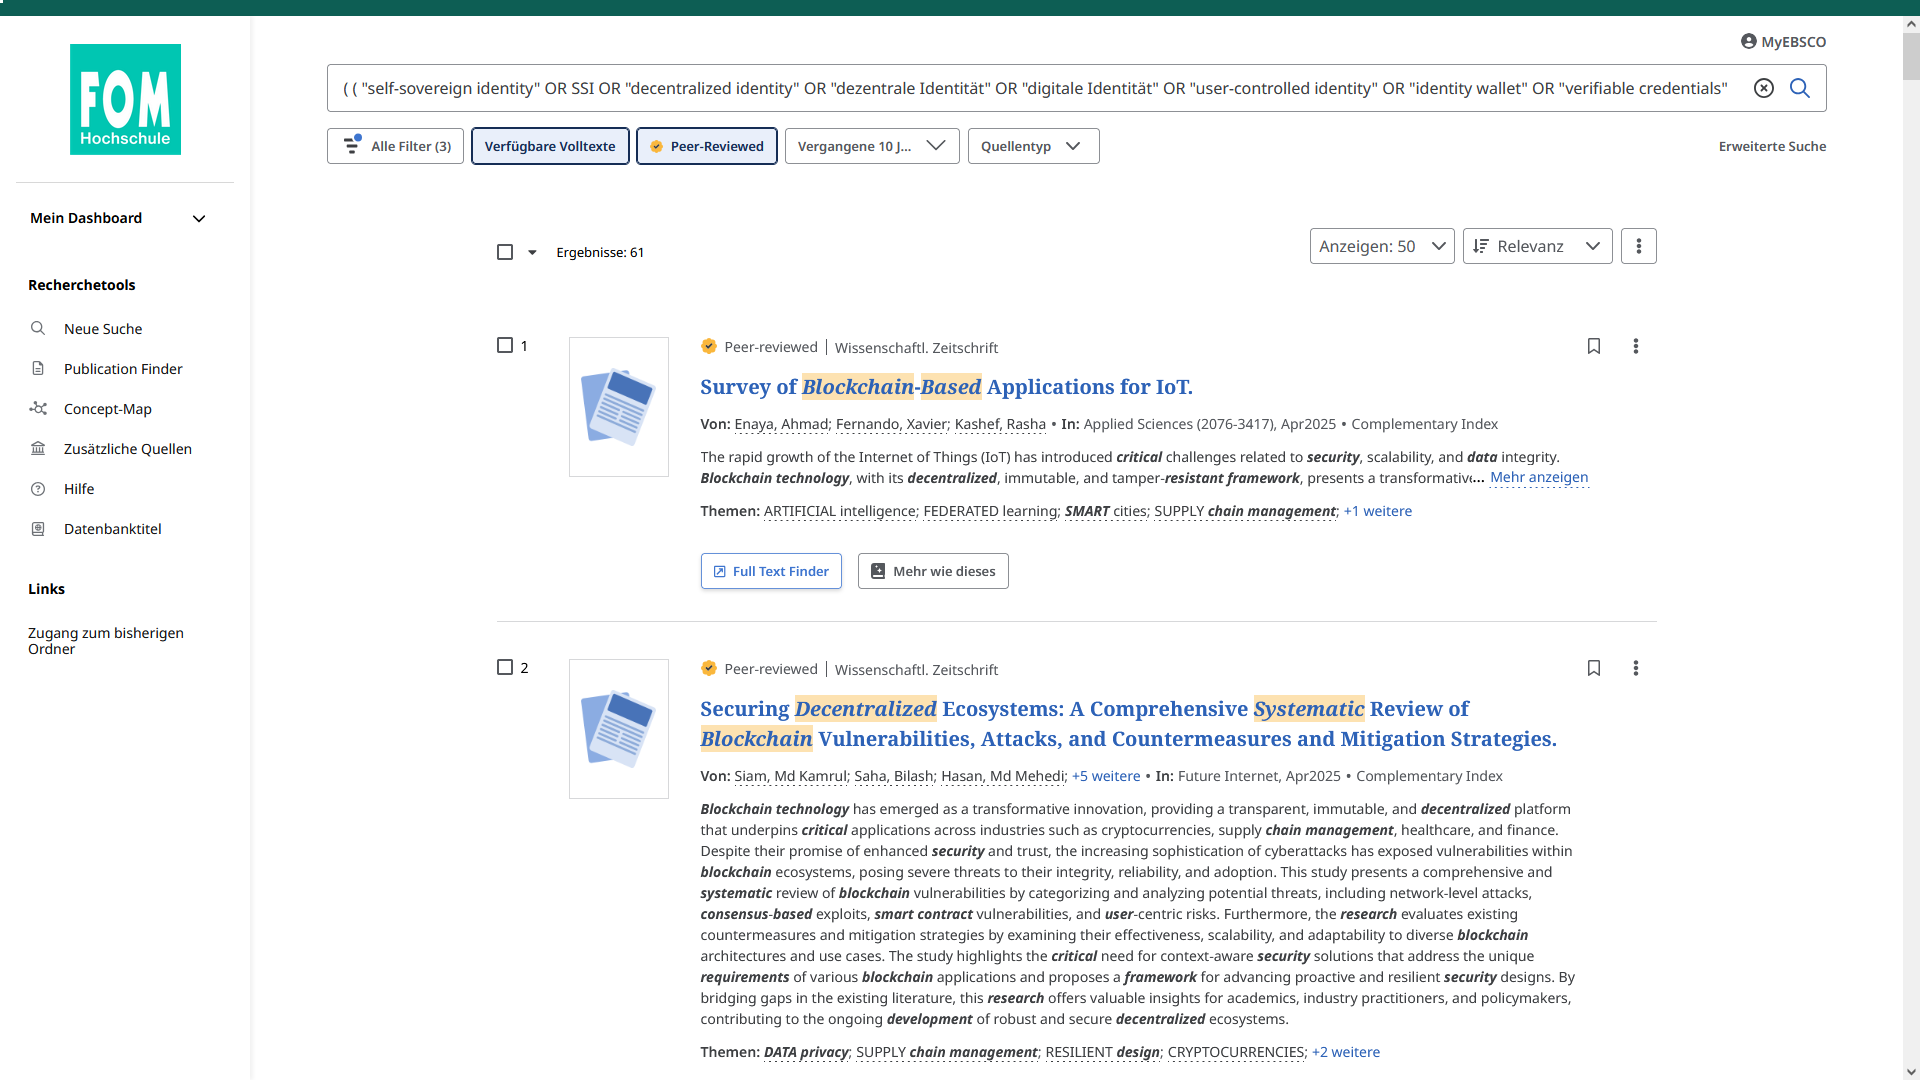
\includegraphics[width=\paperwidth, height=\paperheight, keepaspectratio, angle=90]{EBSCO.png}
    \caption{Ergebnis der EBSCO Suchanfrage}
    \begin{flushleft}
    \textit{Anmerkung.} Eigene Darstellung.
    \end{flushleft}
    \label{fig:EBSCO Ergebnis}
\end{figure}

\paragraph*{Bewertung der Ergebnisse}

\autoref{tab:quellenuebersicht} stellt eine Übersicht der Bewertung der 61 identifizierten Quellen dar, welche vollständig in \ref{sec:Anhang_Systematische Literaturrecherche} aufzufinden ist.

Die Einstufung basiert auf Titel und Abstract in Bezug auf den thematischen Fokus der Arbeit. Hohe Relevanz erhalten Quellen mit klaren Beiträgen zu \ac{SSI}, \ac{PQC}, \ac{KRITIS} oder dezentralen Identitätsarchitekturen. Mittlere Relevanz wird Arbeiten zugeordnet, die angrenzende Technologien wie Blockchain-Sicherheit im \ac{IoT} oder digitale Forensik behandeln. Niedrige Relevanz erhalten Quellen zu allgemeinen Technologietrends ohne direkten Bezug zum Thema.

\begin{longtable}{L{1.5cm}L{11cm}L{1cm}}
    \caption[]{Übersicht der Bewertung der identifizierten Quellen hinsichtlich ihrer Relevanz}
    \label{tab:quellenuebersicht} \\
    \toprule
    \textbf{Nr.} & \textbf{Quelle} & \textbf{Relevanz} \\
    \midrule
    \endfirsthead
    \multicolumn{3}{l}{\textit{Tabelle \thetable\ (Fortsetzung)}} \\
    \toprule
    \textbf{Nr.} & \textbf{Quelle} & \textbf{Relevanz} \\
    \midrule
    \endhead
    \midrule
    \multicolumn{3}{r}{\textit{Fortsetzung auf nächster Seite}} \\
    \endfoot
    \bottomrule
    \multicolumn{3}{p{\linewidth}}{\textit{Anmerkung.} Basierend auf \autoref{tab:quellenbewertung} und Titel und Abstracts von \textcite{szymanski_QuantumSafeSoftwareDefinedDeterministicInternetThingsIoTHardwareEnforcedCyberSecurityCriticalInfrastructures_2024,nouma_TrustworthyEfficientDigitalTwinsPostQuantumEraHybridHardwareAssistedSignatures_2024,sharif_EIDASRegulationSurveyTechnologicalTrendsEuropeanElectronicIdentitySchemes_2022,alam_PrivatelyGeneratedKeyPairsPostQuantumCryptographyDistributedNetwork_2024,radanliev_ReviewComparisonUSEUUKRegulationsCyberRiskSecurityCurrentBlockchainTechnologies_2023}.} \\
    \endlastfoot
    1 & Szymanski, T. H. (2024). A Quantum-Safe Software-Defined Deterministic Internet of Things (IoT) with Hardware-Enforced Cyber-Security for Critical Infrastructures. Information (2078-2489), 15(4), 173. \url{https://doi.org/10.3390/info15040173} & Hoch \\
    \midrule
    2 & Nouma, S. E., \& Yavuz, A. A. (2024). Trustworthy and Efficient Digital Twins in Post-Quantum Era with Hybrid Hardware-Assisted Signatures. ACM Transactions on Multimedia Computing, Communications \& Applications, 20(6), 1–30. \url{https://doi.org/10.1145/3638250} & Hoch \\
    \midrule
    3 & Sharif, A., Ranzi, M., Carbone, R., Sciarretta, G., Marino, F. A., \& Ranise, S. (2022). The eIDAS Regulation: A Survey of Technological Trends for European Electronic Identity Schemes. Applied Sciences (2076-3417), 12(24), 12679. \url{https://doi.org/10.3390/app122412679} & Hoch \\
    \midrule
    4 & Alam, M., Hoffstein, J., \& Cambou, B. (2024). Privately Generated Key Pairs for Post Quantum Cryptography in a Distributed Network. Applied Sciences (2076-3417), 14(19), 8863. \url{https://doi.org/10.3390/app14198863} & Hoch \\
    \midrule
    5 & Radanliev, P. (2023). Review and Comparison of US, EU, and UK Regulations on Cyber Risk/Security of the Current Blockchain Technologies: Viewpoint from 2023. Review of Socionetwork Strategies, 17(2), 105–129. \url{https://doi.org/10.1007/s12626-023-00139-x} & Hoch \\
    \midrule
    6--38 & Diverse & Mittel  \\
    \midrule
    39--61 & Diverse & Niedrig \\
\end{longtable}